\documentclass[a4paper,12pt,oneside,final]{memoir}
% Cl.7/2 - 1.5x line spacing
%\OnehalfSpacing

%%%%%%%%%%%%%%%%%%%%%%%%%%%%%%%%%%%%%%%%%%%%%%%%%%%%%%%%%%%%%%%%%%%%%%%%%%%%%%%%
% Page geometry
%%%%%%%%%%%%%%%%%%%%%%%%%%%%%%%%%%%%%%%%%%%%%%%%%%%%%%%%%%%%%%%%%%%%%%%%%%%%%%%%
% Cl.7/3 - 3.5cm left, 2cm right
\setlrmarginsandblock{3.5cm}{2cm}{*}
% Cl.7/3 - 2.5cm left, 2.5cm right
\setulmarginsandblock{2.5cm}{2.5cm}{*}
\checkandfixthelayout
\usepackage[slovak]{babel}
%\usepackage{fontspec}
% \usepackage[slovak]{babel}
\usepackage{microtype} % Typographical improvements
\usepackage[bottom]{footmisc} % Move footnotes to the bottom
\usepackage{epsfig}
\usepackage{epstopdf}
\usepackage[chapter]{algorithm}
\usepackage[chapter]{minted}
\usepackage{algorithmic}
\usepackage{listings}
\usepackage{amsmath}
\usepackage{graphicx}
\usepackage{multirow}
\usepackage{color}
\usepackage{url}
\usepackage[utf8]{inputenc}
\usepackage{url}
\usepackage{pdfpages}
\usepackage{fixltx2e}
\usepackage[chapter]{minted}
\usemintedstyle{tango}
\renewcommand\listingscaption{Source}
\addto\captionsslovak{\renewcommand{\contentsname}{Table of Contents}}
\addto\captionsslovak{\renewcommand{\listfigurename}{List of Figures}}
\addto\captionsslovak{\renewcommand{\bibname}{References}}
\addto\captionsslovak{\renewcommand{\chaptername}{Chapter}}
\addto\captionsslovak{\renewcommand{\figurename}{Fig.}}
\renewcommand\baselinestretch{1.5} % riadkovanie jeden a pol

% pekne pokope definujeme potrebne udaje
\def\mftitle{Light transport visualization and perturbations}
\def\mfthesistype{Baccalaureate Thesis}
\def\mfauthor{Martin Pinter}
\def\mfadvisor{Prof. RNDr. Roman Ďurikovič, PhD.}
\def\mfplacedate{Bratislava, 2014}

\ifx\pdfoutput\undefined\relax\else\pdfinfo{ /Title (\mftitle) /Author (\mfauthor) /Creator (PDFLaTeX) } \fi

\begin{document}

\frontmatter

\thispagestyle{empty}

\noindent
\begin{minipage}{\textwidth}
\begin{center}
\uppercase{Comenius University in Bratislava \\
Faculty of Mathematics, Physics and Informatics}
\end{center}
\end{minipage}

\vfill
\begin{center}
\begin{minipage}{0.8\textwidth}
\center{\textbf{\LARGE\MakeUppercase{\mftitle}}}
\smallskip
\centerline{\mfthesistype}
\end{minipage}
\end{center}
\vfill
2014 \hfill
\mfauthor
\eject 
% koniec obalu

\thispagestyle{empty}

\begin{minipage}{\textwidth}
\begin{center}
\uppercase{Comenius University in Bratislava \\
Faculty of Mathematics, Physics and Informatics}
\end{center}
\end{minipage}

\vfill
\begin{center}
\begin{minipage}{0.8\textwidth}
\centerline{\textbf{\MakeUppercase{\mftitle}}}
\smallskip
\centerline{\mfthesistype}
\end{minipage}
\end{center}
\vfill
\begin{tabular}{l l}
%Registration number: & 40a99bd8-3cb6-4534-9330-c7fd9b5e5ca4 \\ podla vsetkeho toto v bakalarke netreba
Study programme: & Informatics\\
Branch of study: & 2508 Informatics\\
Educational facility: & Department of Informatics\\
Supervisor: & \mfadvisor
\end{tabular}
\vfill
\mfplacedate \hfill
\mfauthor
\eject 
% koniec titulneho listu

\thispagestyle{empty}
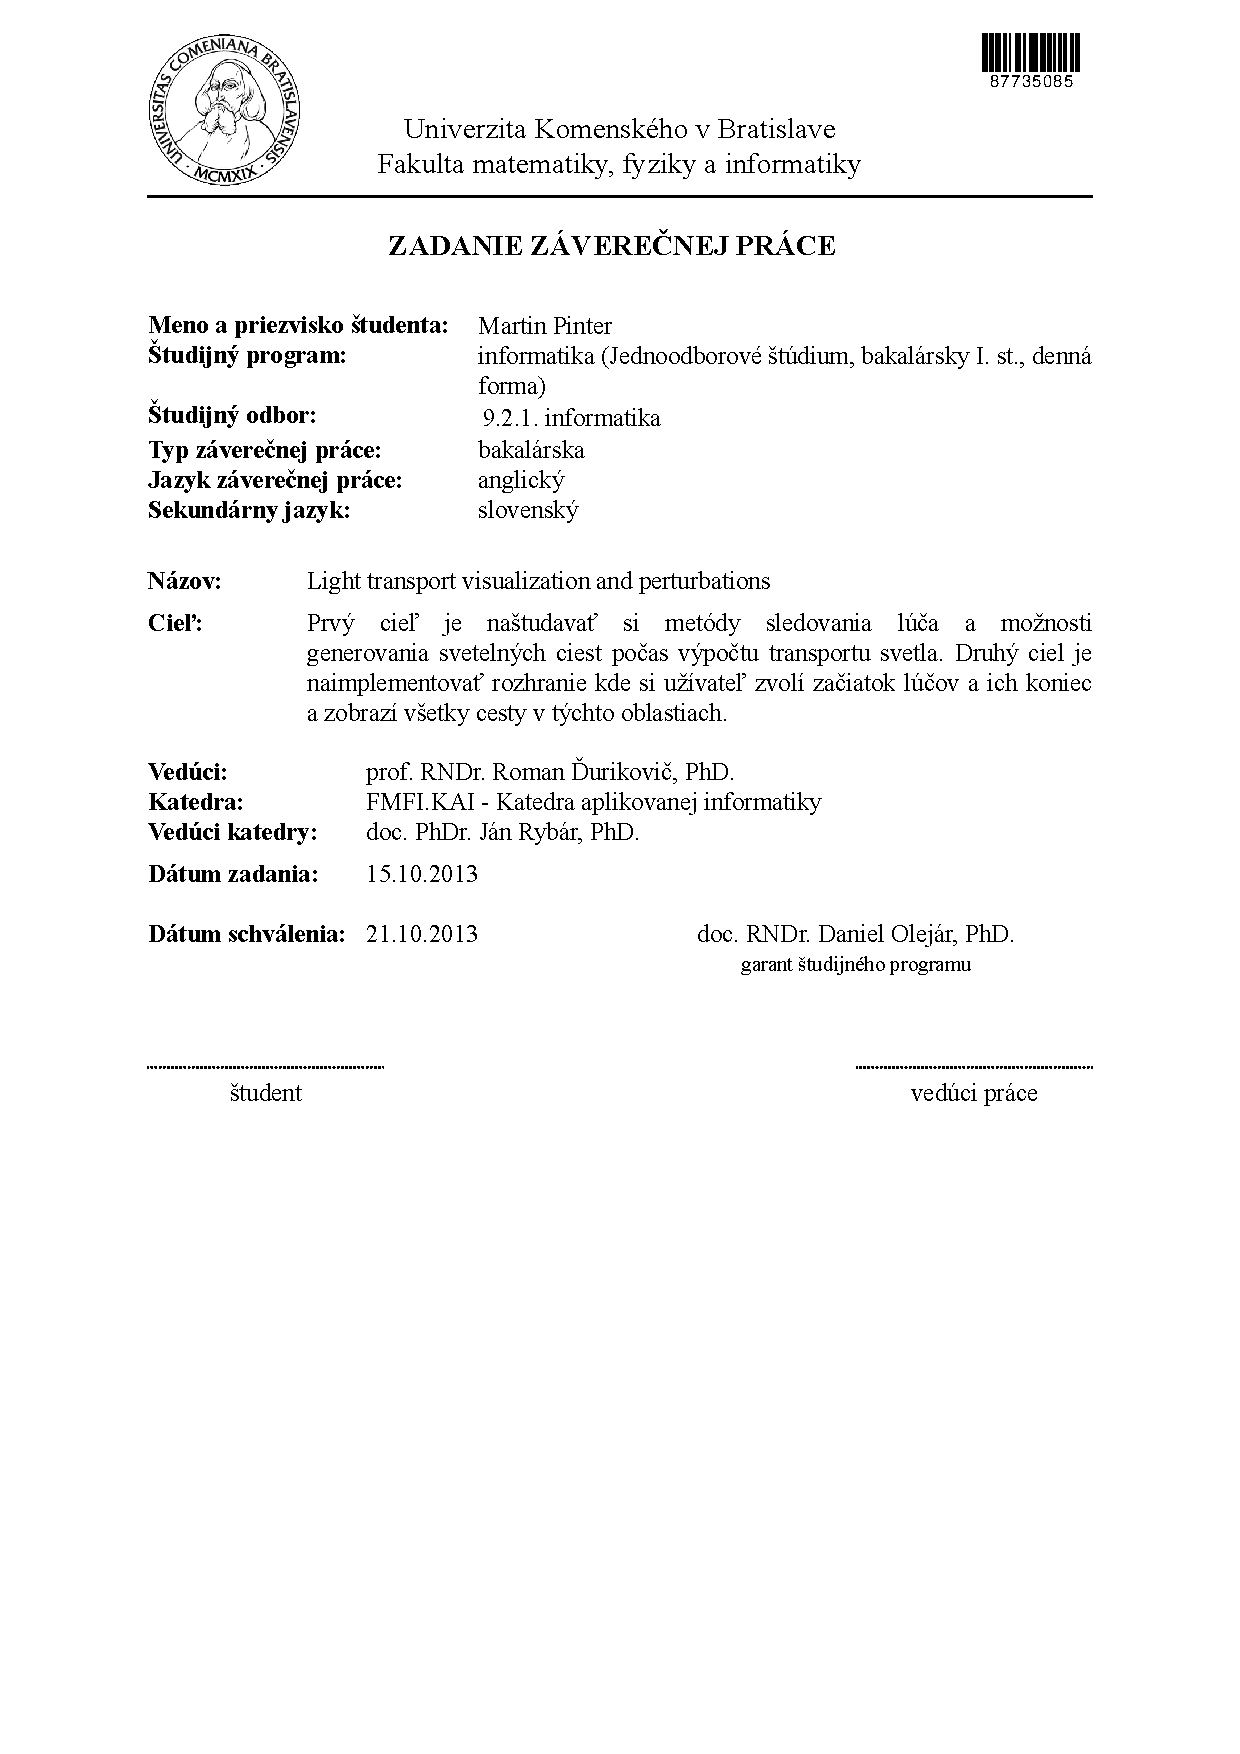
\includepdf[pages=1]{zadanie.PDF}
\vfill
\eject
% koniec zadania

%prihlaska tu ?

%\thispagestyle{empty}

%{~}\vspace{12cm}

%\noindent
%\begin{minipage}{0.25\textwidth}~\end{minipage}
%\begin{minipage}{0.75\textwidth}
%I hereby declare that all parts of this thesis have been written by myself using only the references explicitly referred to in the text and consultations with my supervisor.
%\newline \newline
%\end{minipage}
%\vfill
%~ \hfill {\hbox to 6cm{\dotfill}} \\
%\mfplacedate \hfill Martin Pinter
%\vfill\eject 
% koniec prehlasenia

%\includepdf[pages={1}]{prihl.pdf}

\chapter*{Acknowledgements}\label{chap:thank_you}
I would like to thank my advisor \mfadvisor for his guidance and invaluable advice throughout my work on this thesis. I would also like to thank my colleagues from YACGS seminar for useful tips regarding the implementation. Finally, I want to thank my family and friends for their support and encouragement during my studies.
\vfill\eject 

\chapter*{Abstrakt}\label{chap:abstract_sk}
Práca sa zaoberá algoritmami prenosu svetla a sledovania lúčov, pričom sa sústreďuje najmä na Metropolis light transport. Spomínané sú variácie tohto algoritmu, vychádzajúce z myšlienok pôvodného článku publikovaného v roku 1997. Predstavená je knižnica umožňujúca interaktívnu vizualizáciu algoritmov prenosu svetla v reálnom čase, ktorá tiež umožní používatelovi filtrovať jednotlivé lúče zvolením oblasti ktorou má lúč prechádzať. Taktiež umožní sledovať perturbácie zvoleného lúča podľa pravidiel MLT-algoritmu a jeho mutačných stratégií.

~\\
Kľúčové slová: Metropolis Light Transport, global illumination, vizualizácia, OpenGL
\vfill\eject 

\chapter*{Abstract}\label{chap:abstract_en}
Thesis revolves around methods of path-tracing and light-transport in computer graphics, with its main focus on Metropolis light transport. It lists through algorithms that spawned from the initial idea of MLT published in 1997, then presents a library for real-time interactive visualization of light-transport algorithms, that allows users to filter through light paths generated by the raytracer by selecting an area through witch the light path that he wishes to visualize must pass. The library also offers a visualization of perturbations according to the Metropolis framework and mutation strategy of the given algorithm.

~\\
Keywords: Metropolis Light Transport, global illumination, visualization, OpenGL
\vfill\eject 
% koniec abstraktov

\chapter*{Foreword}\label{chap:foreword}
While never being at the forefront of computer graphics research, the idea of Metropolis Light Transport has been kept alive since its first incarnation, with a decent number of works improving on the original notion. Lately, the interest seems to have resurged, with derivative works showing up on both SIGGRAPH 2012 and 2013. Yet, visualization tools are practically non-existent, not only for MLT based algorithms, but also for ray or path tracing as a whole (the best tool probably being a plugin for 3DS Max, designed primarily to allow light path manipulation for 3d artists). This work aims to round up the theory behind MLT, focusing on the original concept but also mentioning the various improvements, and to create a basic tool for visualization of light paths, and light path mutations. The core of this application will be relying on a tried and tested, widely used graphics libraries, namely Assimp and Mitsuba, with real time visualization in OpenGL. The reader should have at least a very basic background knowledge of methods in computer graphics. 
\vfill\eject 
\begin{KeepFromToc}
	\tableofcontents
	\newpage
	\listoffigures
\end{KeepFromToc}


\mainmatter

\chapter*{Introduction}\label{chap:introduction}
The concept of simulating rays of light to create physically correct, believable and maybe even photorealistic renders of three dimensional scene is not a new one in the computer graphics community. If we take Arthur Appels work on ray casting as a basis, then the idea itself is almost half a century old. Over the years the concept developed and evolved into numerous algorithms and today most of them fall under an umbrella term of global illumination - a name indicating that these algorithms do not account only for light coming directly from a light source (such algorithms, including the original Appels raycasting, would be labeled under a direct illumination moniker), but also for light reflecting off of other surfaces in a scene, whether reflective or not. These include radiosity, photon mapping, ray tracing, path tracing, Metropolis light transport and other.

Today, global illumination algorithms are used in a variety of fields, from design and architecture to film industry. In this setting, every possible optimisation in terms of required time or processing power may have a serious impact on projects budget. And with these algorithms relying mostly on brute force, there are certainly places to improve. Since MLT may be one of the methods that pushes the boundaries again - and it has already successfully done so in the recent years - having tools to experiment with it should be beneficial. 

Apart from providing a round up of theoretical knowledge in the field, this work is to provide a visualisation library for the MLT algorithm (and possibly for any other path tracing technique). The main challenge would be to visualise the data usually produced by an offline renderer in a real time interactive environment (OpenGL). The application also aims to be platform independent, using only widely supported, cross-platform libraries and methods.

\input 01intro.tex
\input 02visualisation.tex
\input 05results.tex
\input 06conclusion.tex

\backmatter

\nocite{*}
\bibliographystyle{alpha}
\bibliography{research}

\end{document}
